% !TeX root = ../main.tex

\chapter{基于事件相机的火焰特征提取}
基于事件相机的火焰特征提取工作主要在于对提取的事件帧图象进行相关的图像学处理,从中提取出能够用来
描述火焰轮廓,图形特征的有关参数指标,这些数值参数构成的多维向量将会作为检测算法中用于分类的重要
依据,本章便是对本次工作中相关提取算法的搭建原理与流程进行一个全面介绍。

\section{火焰特征}
火焰的特征包括静态和动态,通常可以按如图\ref{5}所示的方式分类
\begin{figure}
    \centering
    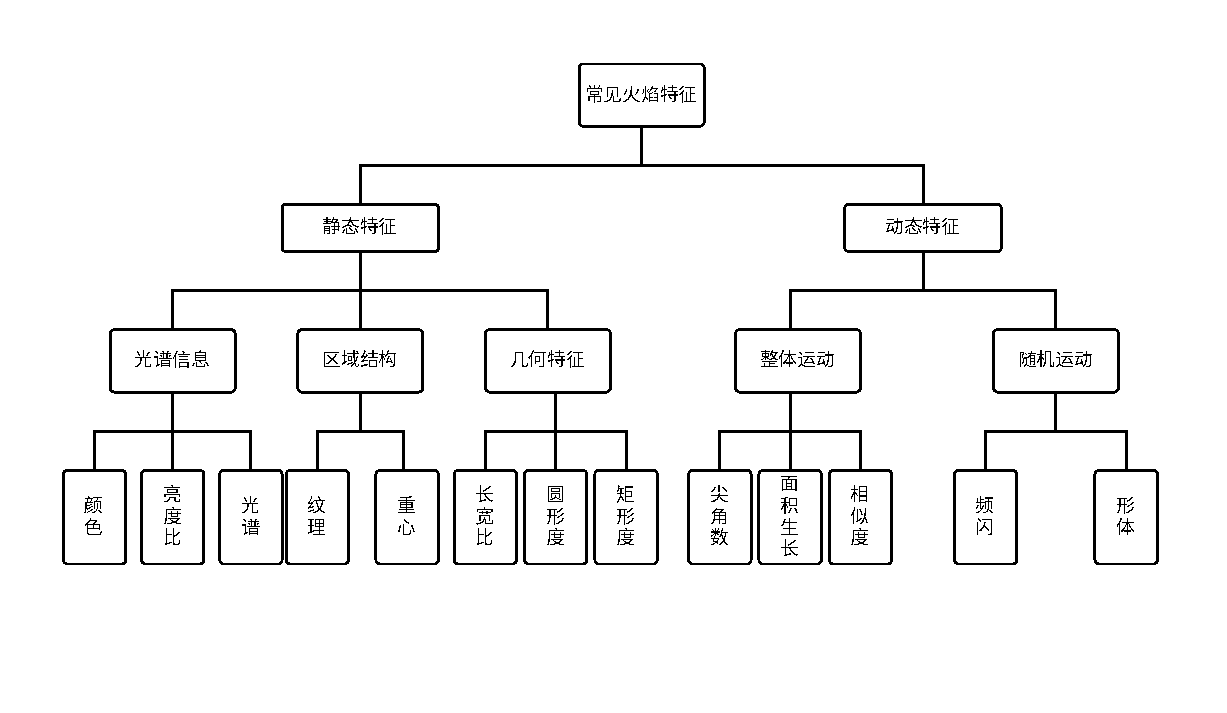
\includegraphics[width=\textwidth]{figures/extract_characteristic.pdf}
    \caption{火焰特征分类}
    \label{5}
\end{figure}

\subsection{事件数据的预处理}
我们在第二章对相关原理的介绍中已经提到,事件数据是一种新颖的数据类型,对其的处理方法也与传统视觉处理方法不同。
事件相机拍摄的视频图像,以原始的DVS数据格式转换为时空格式储存,每条事件数据包括了四类信息:事件在相机二维平面的坐标,
事件发生时的时间,事件的极性。为了与目前常见的的计算机视觉算法相适配,我们预处理的工作便是将事件数据转换为类似二维平面图像
的形式,从而适应后续的机器学习训练。预处理将按照下列步骤进行:

步骤一:滤除多余事件。在第三章数据集的制作工作中,我们对火焰图像进行了人工标定,并框出了其具体的位置坐标,对于出现在
框外的事件来讲,就属于无用的冗杂信息,我们可以利用手工框的坐标,将不在范围内发生的事件进行剔除,大大减少后续的计算量。效果展示如图\ref{14}。
\begin{figure}[ht]
    \centering
    \begin{subfigure}{0.49\textwidth}
        \centering
        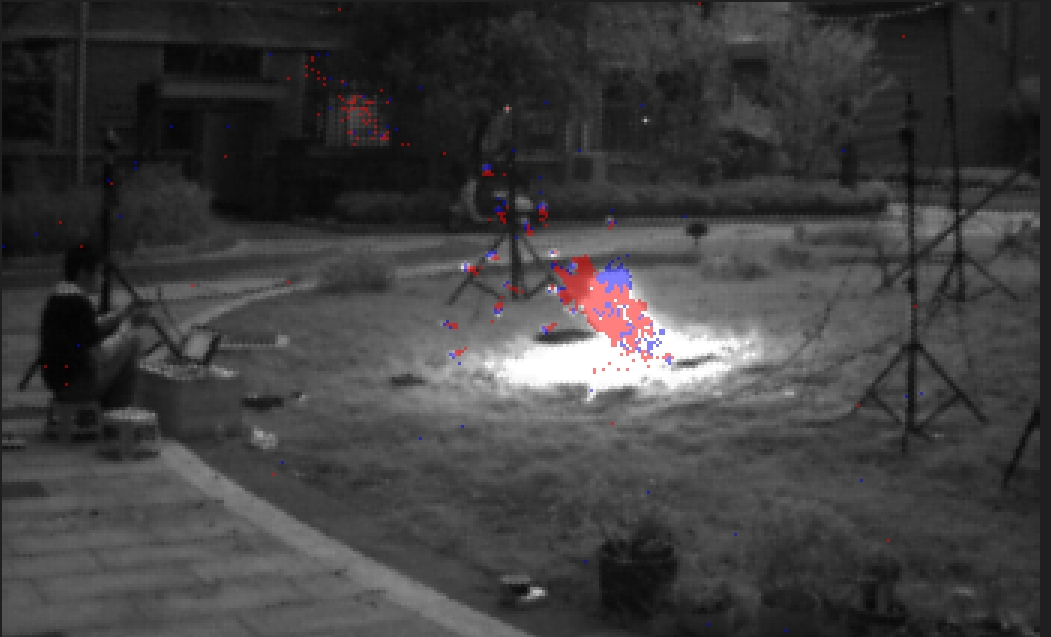
\includegraphics[width=\textwidth]{figures/extract_process_01.png}
        \caption{原始数据}
        \label{14.a}
    \end{subfigure}
    \hfill
    \begin{subfigure}{0.49\textwidth}
        \centering
        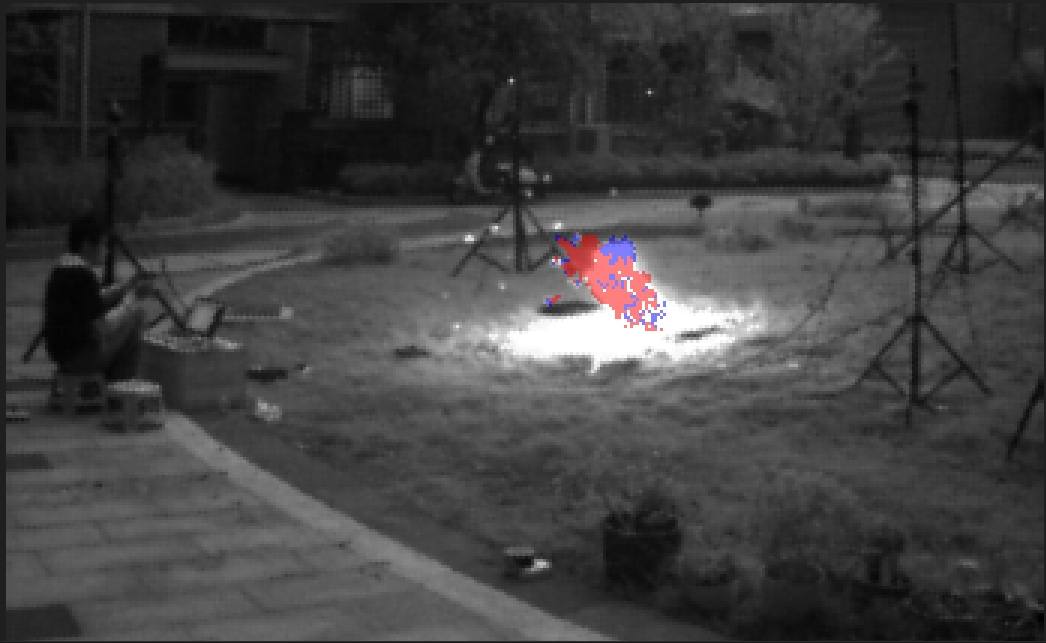
\includegraphics[width=\textwidth]{figures/extract_process_02.png}
        \caption{滤除后数据}
        \label{14.b}
    \end{subfigure}
    \caption{滤除多余事件}
    \label{14}
\end{figure}

步骤二:在数据集的制作工作中,我们已经按照33ms的时间窗口,将时间序列划分为多个片段,每个片段都严格按照事件发生的空间信息将事件
投影在对应位置的像素上,形成二维的二值图像,即我们的事件帧图像。这里类似的,我们仍以33ms作为事件的时间窗口,将步骤一处理后的事件数据
按照同样的思路进行像素投影得出二值图像。效果展示如图\ref{15}。

\begin{figure}[ht]
    \centering
    \begin{subfigure}{0.49\textwidth}
        \centering
        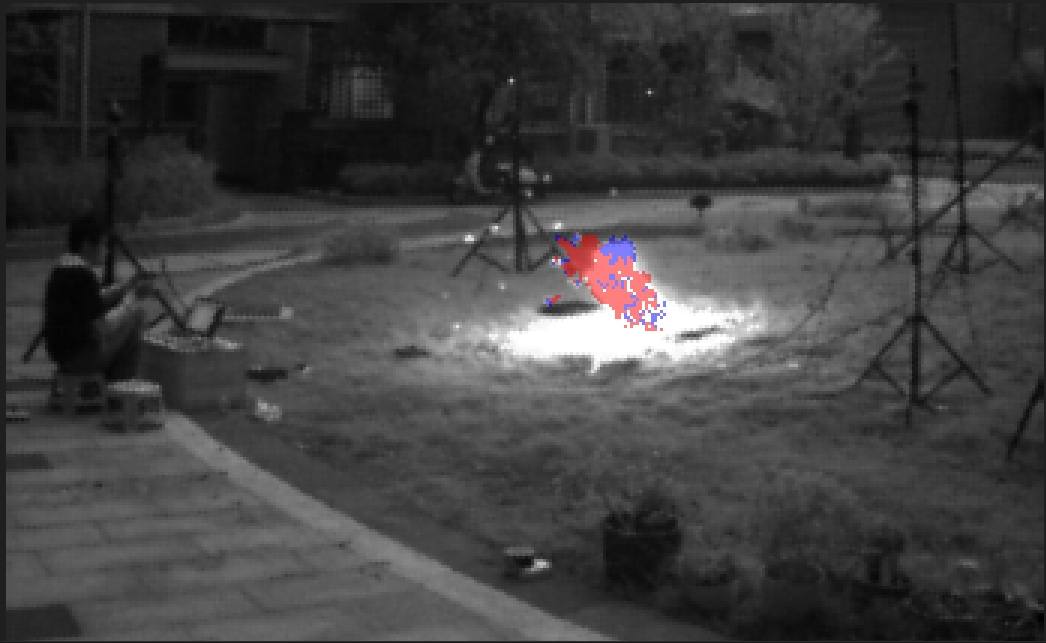
\includegraphics[width=\textwidth]{figures/extract_process_02.png}
        \caption{滤除后数据}
        \label{15.a}
    \end{subfigure}
    \hfill
    \begin{subfigure}{0.49\textwidth}
        \centering
        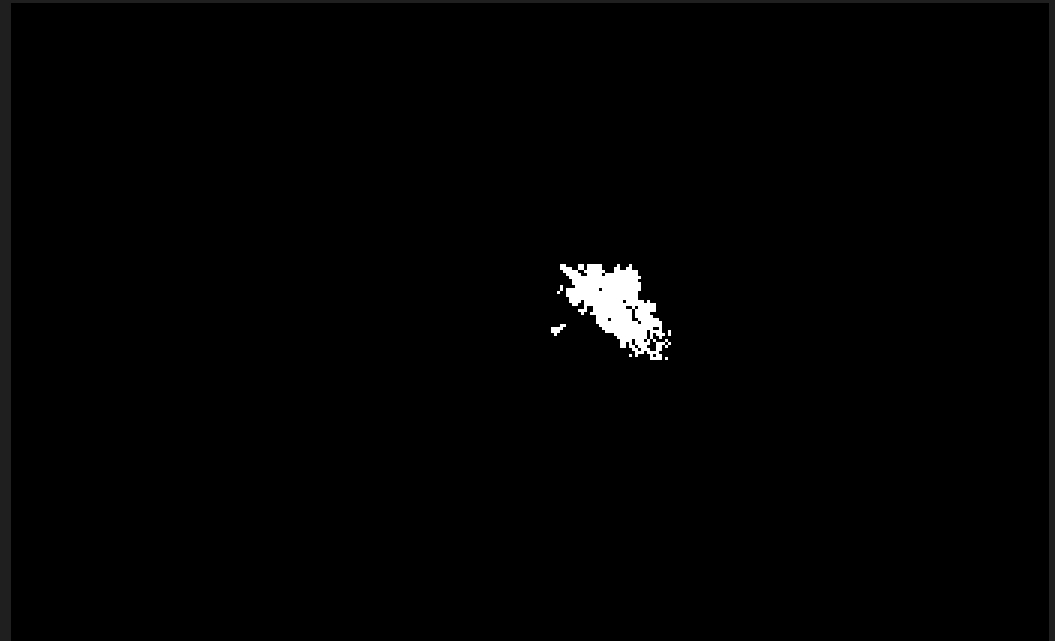
\includegraphics[width=\textwidth]{figures/extract_process_03.png}
        \caption{投影后二值图}
        \label{15.b}
    \end{subfigure}
    \caption{投影}
    \label{15}
\end{figure}

步骤三:去噪工作,这里利用到的是形态学的膨胀腐蚀操作,两者都是对二值化黑白图像的常用处理手段。膨胀用于扩展图像中的白色区域。它通过在图像中滑动一个结构元素(通常是一个矩形内核),将内核覆盖的区域内的所有像素设为白色。如果该区域内至少有一个白色像素存在,则该区域即被视为白色。这一操作往往是填充小空洞,连接断裂或相邻,扩展边界。腐蚀操作与膨胀相反,它会收缩图像中的白色区域,通过在图像中滑动一个结构元素,将内核覆盖的区域内的所有像素设为白色。只有当该区域内的所有像素都是白色时,该区域才会被保留为白色,否则将被设为黑色,这一操作往往用于去除小物体,分离相邻,缩减图象大小。我们选定了合适的核大小,可以理解为上述操作的步长,先腐蚀去除噪声,再膨胀进行修补,最后图象只保留下了事件团,完成去噪,预处理结束。效果如图\ref{16}所示。

\begin{figure}[ht]
    \centering
    \begin{subfigure}{0.49\textwidth}
        \centering
        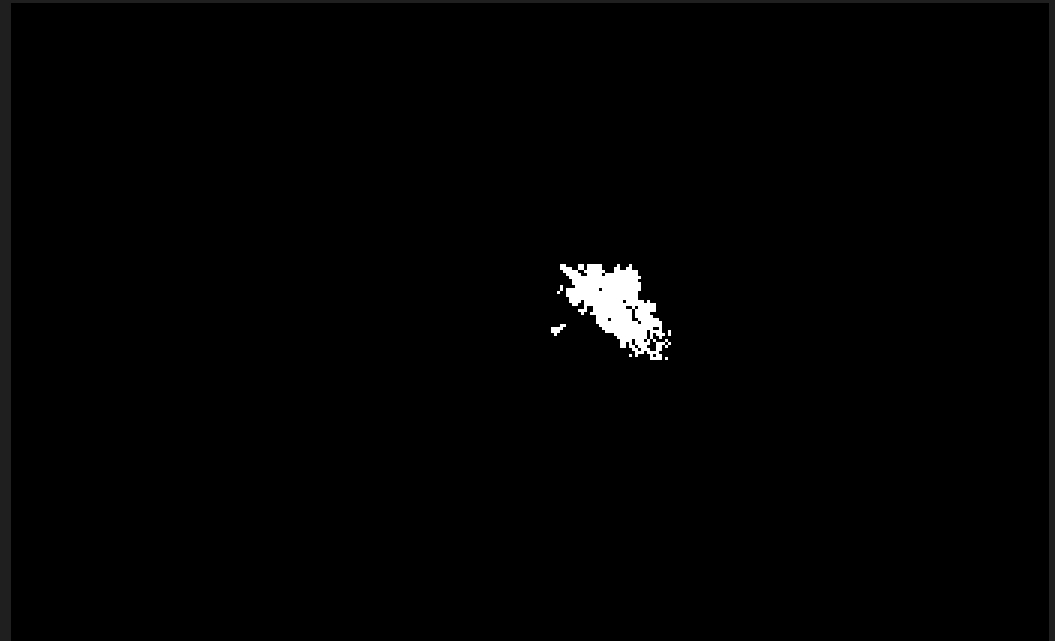
\includegraphics[width=\textwidth]{figures/extract_process_03.png}
        \caption{二值图}
        \label{16.a}
    \end{subfigure}
    \hfill
    \begin{subfigure}{0.49\textwidth}
        \centering
        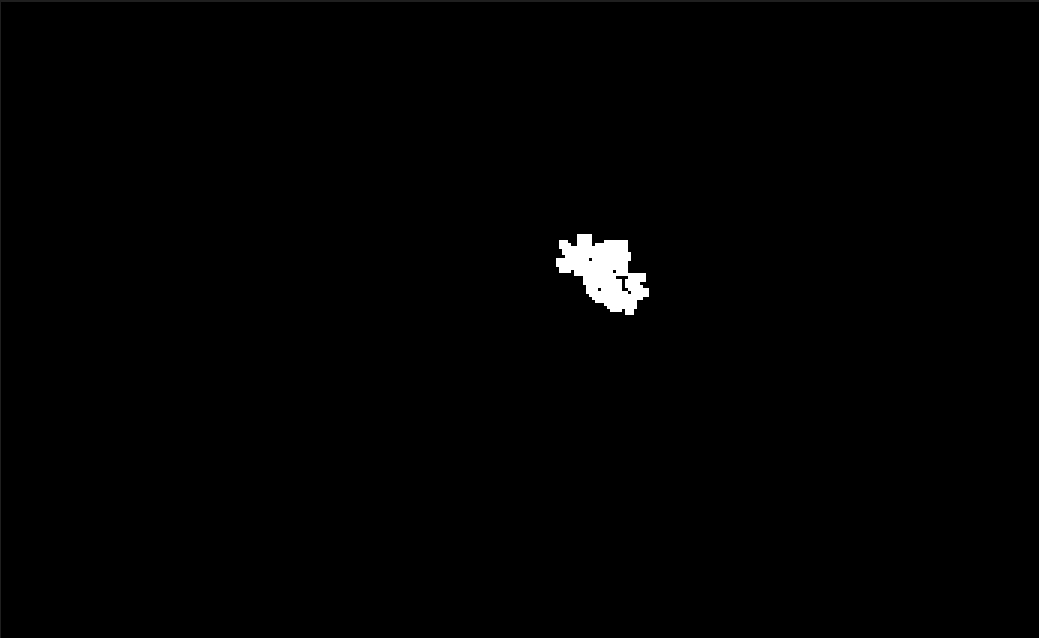
\includegraphics[width=\textwidth]{figures/extract_process_04.png}
        \caption{膨胀与腐蚀后效果}
        \label{16.b}
    \end{subfigure}
    \caption{膨胀与腐蚀}
    \label{16}
\end{figure}

\subsection{火焰的静态特征}
火焰的静态特征主要表征的是图像的空间部分情况,包括较广,颜色,几何特征,纹理都在其范畴内,传统工作中
常常用到的数值参数包括矩形度,圆形度,高度系数等,但是对它们的提取工作并不一定适合事件相机,例如颜色
特征,它反映的是火焰的亮度分布规律,对它的提取一般要对各个颜色通道建立直方图来进行,不适用于本次使用的这台色彩通道单调的事件相机。
这里我们将会根据事件相机的特点,选择或引入有效的,合适的特征数值,作为我们的后续工作的数据基础。

事件输出率,这是我们引入的一个新的静态特征概念,事件相机的特性决定它只会对变化产生响应,如果我们的设备保持
静止不移动的状态,理论上来讲,事件团越密集,发生事件数越多的区域越可能是疑似的火点,那么,我们就可以尝试在一段时间间隔内
计算这个事件的输出频率,为它设置一个阈值来区分火焰与非火焰。假设我们按照一定的时间间隔$\Delta T$(第三章数据集中是33ms)
将时间序列分割成n个小片段,那么在其中第i个片段中,它的某个像素$X_k=(x_k,y_k)$位置在这时间范围$\Delta T$内发生了$n_i,_k(t)$次事件,就可以记做

\begin{equation} 
    out_i,_k=\int_{(i-1)\Delta T}^{i\Delta T} n_i,_k(t) dt
\end{equation}

对它的所有像素进行一个求和,就可以得出在这个时间范围内该片段累积的事件输出总量,写做
\begin{equation} 
    out_i=\sum_{k}out_i,_k=\sum_{k}\int_{(i-1)\Delta T}^{i\Delta T} n_i,_k(t) dt
\end{equation}


定义事件输出率$R_i$等于累计输出总量$out_i$与时间长度$\Delta T$之比,那么就有
\begin{equation} 
R_i=\frac{out_i}{\Delta T}=\frac{\sum_{k}\int_{(i-1)\Delta T}^{i\Delta T} n_i,_k(t) dt}{\Delta T}
\end{equation}

这就是事件输出率的定义式,我们还可以证明在极短的时间内事件输出率$R_i$与对数亮度梯度$- \nabla L(X,t)$为正比关系,符合火焰特性,这里不再赘述,可参考丁赛喆的工作\cite{ding2023}。我们可以通过提取事件帧的
输出事件数与分割时间间隔计算事件输出率,作为分类的重要参数。

圆形度,用于表征火焰轮廓与圆形的相似程度,是描述几何轮廓的重要参数,一般定义为最小外接圆与图象面积之比,公式表示为
\begin{equation} 
    cir=\frac{4\pi S}{L^2}
\end{equation}

一般来说,越接近1,说明形状越接近于圆,非火焰的规则外界物体更容易有着较高的圆形度。
矩形度定义与圆形度相似,为外接矩形与图形面积之比,公式表示为
\begin{equation} 
    rec=\frac{S}{S_R}
\end{equation}

一般来说,矩形度越接近1,火焰越加不稳定,趋于矩形。我们通过利用opencv的相关函数,如findcontours,提取二进制图像的相关边廓信息,对这
两项指标进行相关的计算提取。

形心坐标与静矩(一阶二阶),形心坐标是一个耳熟能详的概念了,图像学中计算相关的形心往往都是将一个像素块看作一个单位1,从而按照相关的定义
来进行形心和一阶矩的计算,这两项与相对位置联系紧密的参数,是后面动态特征中描述相对位置的变化的重要参量。二阶矩可能相对来说,是一个比较陌生一点的概念,它通常用于计算图像的形状特征,如面积、重心、方向等。二阶矩可以通过图像中的像素位置和亮度值的加权平均来计算。
具体来说,二阶矩包括3个独立的值,分别是二阶矩的归一化中心矩:$\mu_{02},\mu_{11},\mu_{20}$。其中,$\mu_{pq}$定义为:
\begin{equation} 
    \mu_{pq}=\sum_{x}\sum_{y}(x-\overline{x})^p(y-\overline{y})^qI(x,y)
\end{equation}

其中,$\overline{x},\overline{y}$分别是两个空间维度的重心坐标,I(x,y)是该像素(x,y)处的亮度。通过二阶矩,可以计算出图像的面积、重心、方向等形状特征,从而对图像进行描述和比较。在目标检测和跟踪中,二阶矩也是描述和比较不同对象的形状、帮助识别和跟踪目标的重要参数。

此外,还有图象面积,长宽比,轮廓长度等一些过于简单的概念,就不再具体介绍。

\subsection{火焰的动态特征}
火焰的动态特征描述的是火焰的空间结构在时间上的变化规律,这是由于在燃烧过程中,火焰会受到多种因素的共同作用的,其中主要有湍流,热对流,重力等,在这些的共同
复杂作用下,火焰会发生视觉上高频持续的形状变化,这种形状上的不断膨胀收缩,被称为闪烁。对于大多数火焰来讲,闪烁频率为7——10HZ,对火焰动态特征的分析,就一般着眼于对
尖角,形心,面积,频闪特性的动态变化描述。
\subsubsection{尖角动态变化}
火焰的尖角是指火焰在燃烧时产生的尖锐、锋利的边缘或者突出部分。火焰是一种由燃烧产生的气体等离子体,通常呈现出流动、不规则的形状,而火焰的尖角则是火焰边缘突出的部分,
有时候也可以是火焰的边缘形成的尖锐角度。

目前对火焰尖角的提取,通常通过角点提取来进行替代,角点是指在局部区域内,图像的灰度强度或颜色呈现出明显的变化,而这种变化不仅仅是灰度值的变化或颜色的变化,还伴随着像素梯度和边缘曲率的变化。
通常情况下,角点可以反映目标的绝大多数轮廓特征,与尖角不做区分。目前常见的角点检测算法包括 Harris 角点检测、Susan 角点检测、FAST 角点检测等。对于本次工作来讲,Harris 角点检测对旋转、平
移和亮度变化具有一定的不变性,所以对相机位置情和环境光线条件有较好的适应性,所以本次的提取工作中我们采用该方法进行提取。

Harris 角点检测是计算机视觉领域中常用的一种角点检测算法,旨在识别图像中的角点。该算法由 Chris Harris 和 Mike Stephens 在 1988 年提出\cite{harris1988combined},是最早的基于局部图像梯度的角
点检测方法之一。这里我们进行Harris 角点检测的基本原理与流程如下:

首先对图像进行梯度计算,通常使用 Sobel 等算子来计算图像在每个像素位置处的水平和垂直方向的梯度。然后,对于每个像素位置,根据其周围邻域的梯度信息构造自相关矩阵,即 Hessian 矩阵。
Harris 算子使用的是一个 2x2 的自相关矩阵,如式\ref{eqn:1}:

\begin{equation} \label{eqn:1}
    M = \sum_{x, y} w(x, y)
    \begin{bmatrix}
        I_x ^2&I_xI_y\\I_xI_y&I_y ^2
    \end{bmatrix}
\end{equation}

其中,$I_x,I_y$分别是像素位置 (x,y) 处的水平和垂直方向的梯度,w(x,y) 是一个窗口函数,通常是高斯函数。之后,利用自相关矩阵,计算一个角点响应函数来判断该像素位置是否为角点。Harris 角点检测使用的是角点响应函数 
R:
\begin{equation} 
    R=det(M)-k(trace(M))^2
\end{equation}

其中,det(M)是自相关矩阵 M 的行列式,trace(M)是其迹,k 是一个常数。最后,由于Harris检测算法对于尺度变化和噪声敏感度较高,也可能对边缘产生一定的响应,所以一般要进行一个非极大值抑制的操作,
将一些低响应的点剔除,只留下高响应的角点。

通过上述的流程,我们可以提取到每一个事件帧中图像的尖角数,一般来讲,火焰的尖角数范围与常见的规则物体或其他干扰源有着较大不同,所以这一数值参数也往往是火焰识别中所依据的最重要的参数,
直接影响到火焰检测算法的效果和可靠性。

这里,我们以25ms为一个事件帧,统计展示了一个一组序列10s的尖角变化曲线,展示如图\ref{6},\ref{7}。
\begin{figure}[ht]
    \centering
    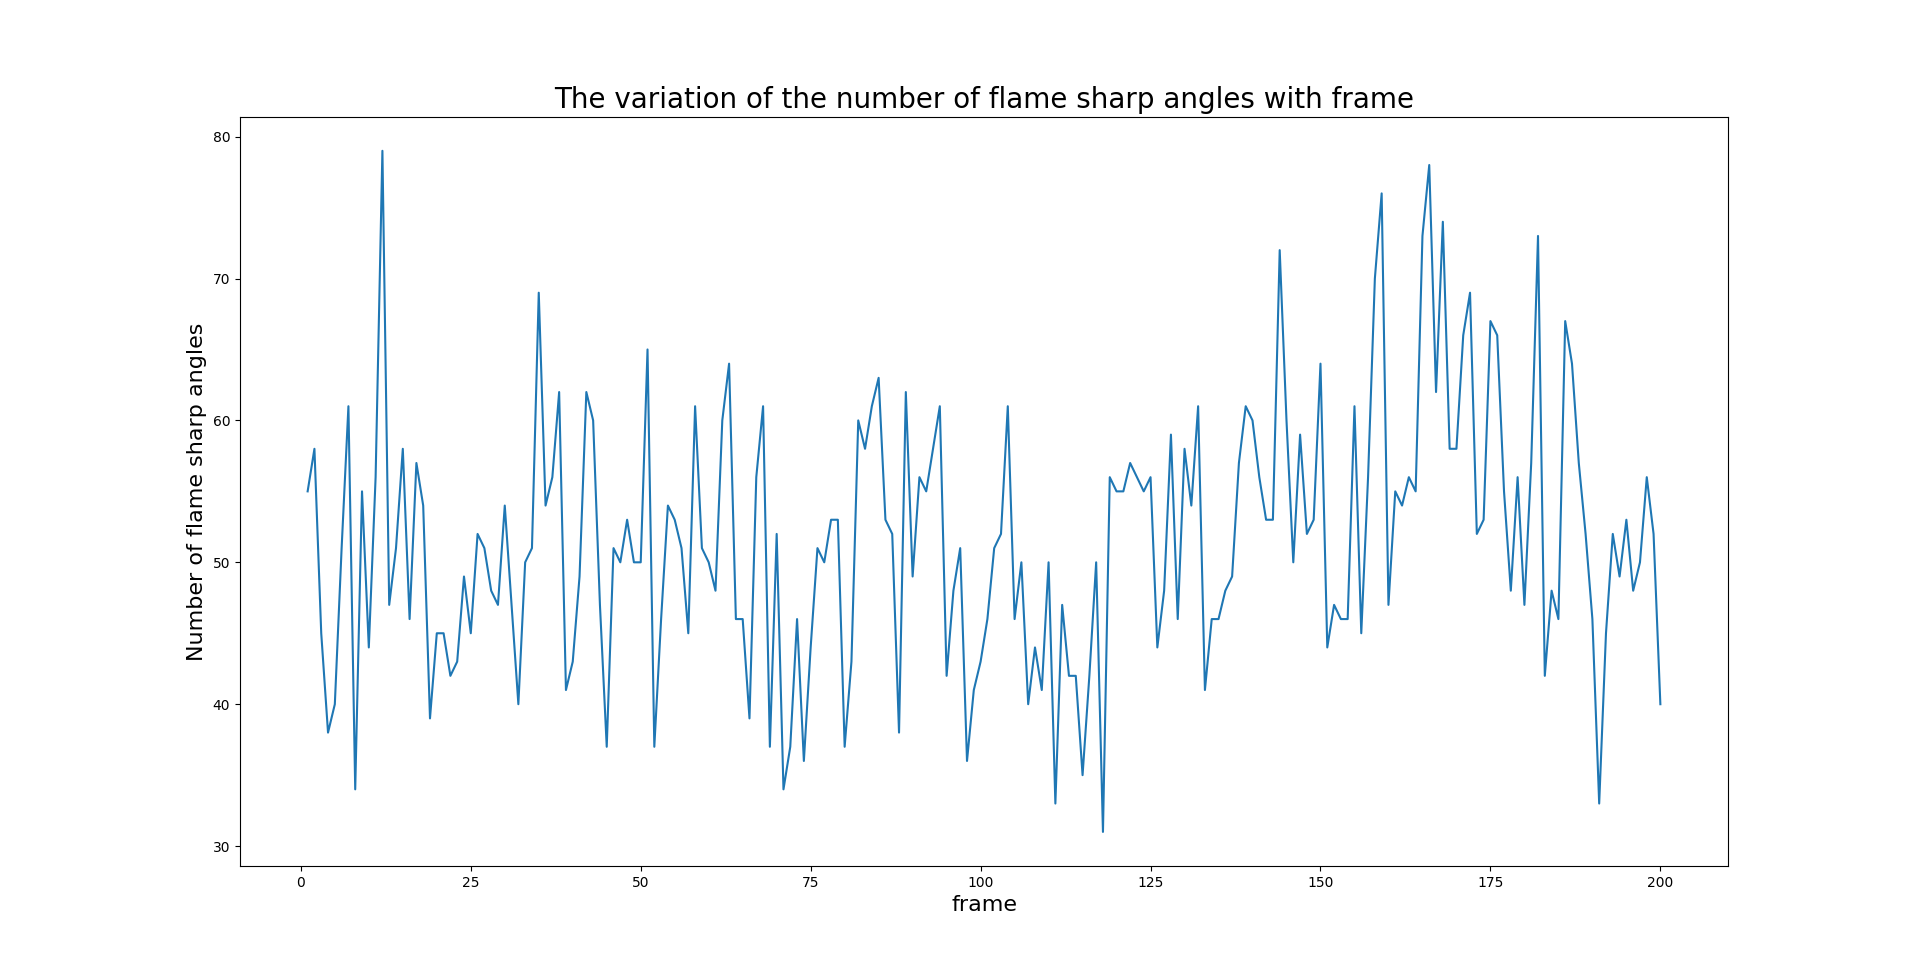
\includegraphics[width=\textwidth]{figures/extract_tip_01.png}
    \caption{0-5s尖角数变化}
    \label{6}
    \end{figure}

\begin{figure}[ht]
    \centering
    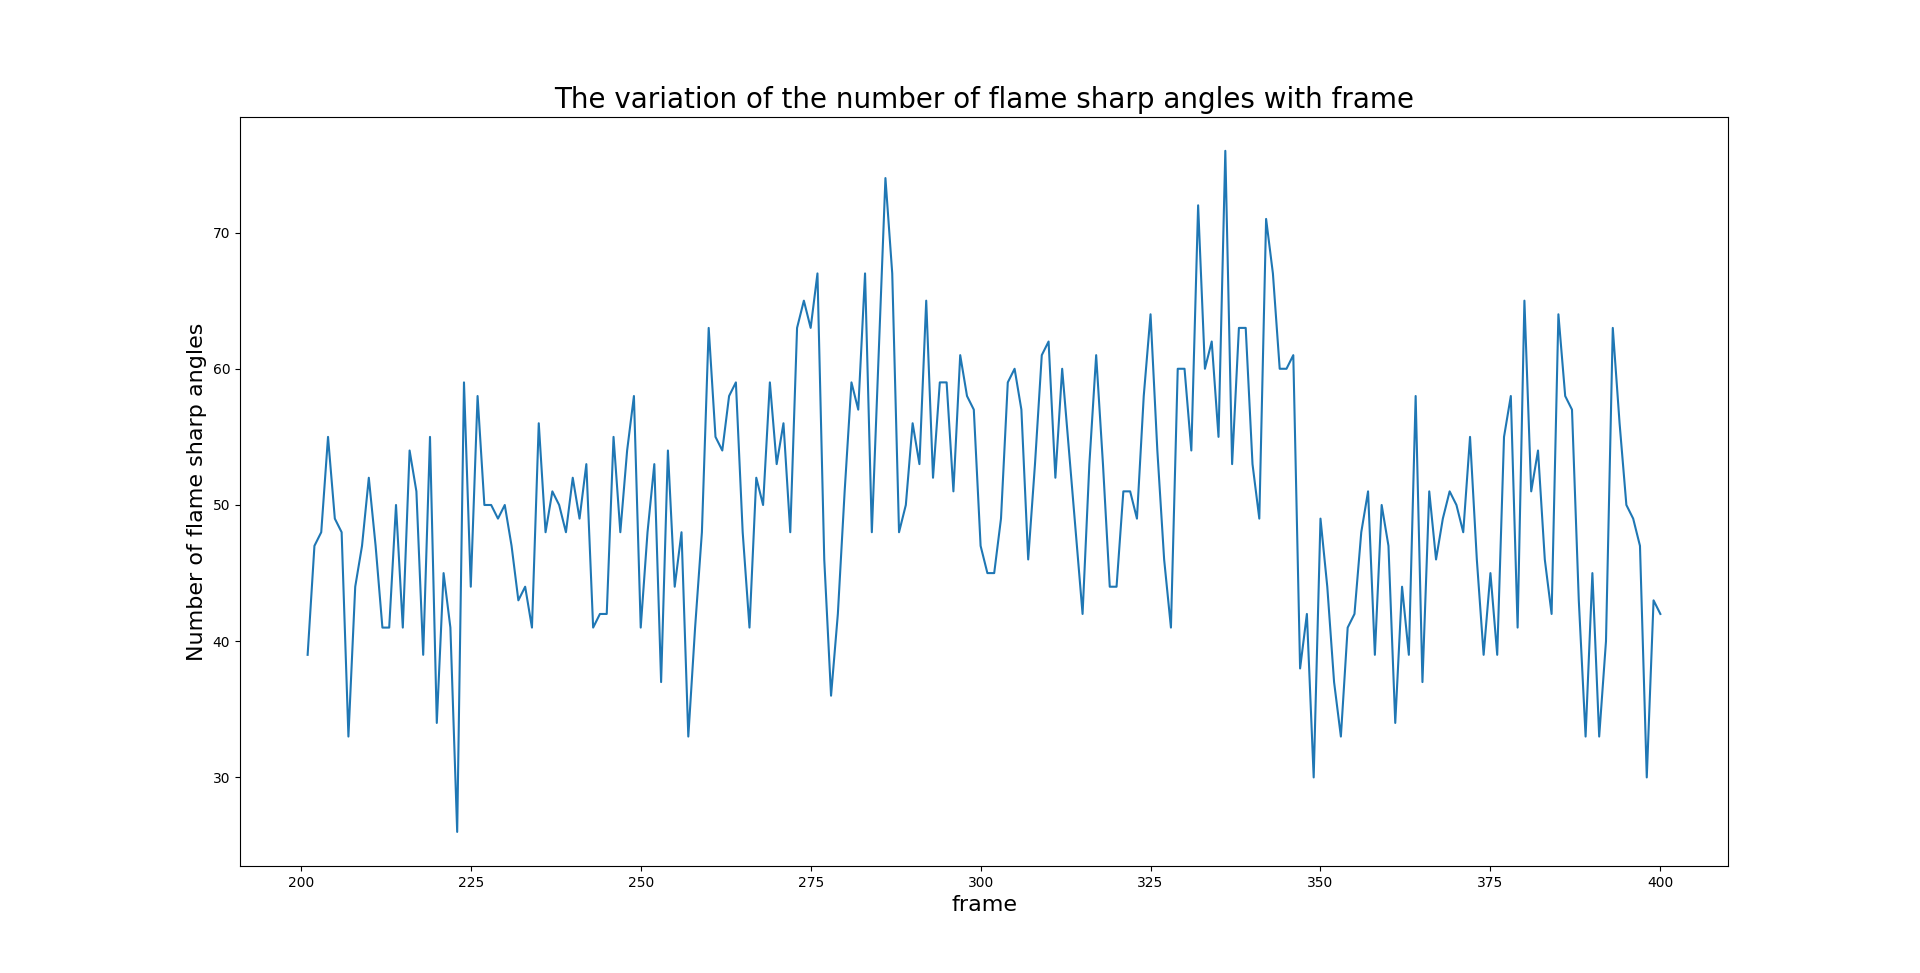
\includegraphics[width=\textwidth]{figures/extract_tip_02.png}
    \caption{5-10s尖角数变化}
    \label{7}
    \end{figure}

火焰图像数据的尖角数往往都在一定的范围内发生无规律非线性的波动,但是按照火焰的时期发展顺序,从火焰的初始燃烧时期到接近熄灭时期,总体趋势上遵循先增后减,符合火焰发展时期的基本特性。

\subsubsection{火焰频闪特性}
火焰的频闪特性是指火焰在燃烧过程中发生周期性变化的现象。这种周期性变化通常以一定的频率进行,即火焰频闪频率。火焰频闪特性是火焰燃烧过程中多种复杂因素相互作用的结果,
这些因素包括燃料供应的不稳定性、燃烧反应的动力学过程、火焰的热传导等,都可能影响这种周期性变化。其中,由于湍流火焰的闪烁而造成火焰边缘的不规则变化理论上也可作为火焰识别算法的
一个依据。根据前面学者的研究,火焰燃烧频率大概在0-12HZ,且这种周期性变化并非线性趋势,而是存在振荡。

由于火焰频闪变化具有不确定性,所以将其作为检测依据的方法目前并不成熟,检测效果也往往不尽人意,往往作为补充参考而存在。
目前对他的研究也分很多不同的方向途径,目前的相关方向着眼于多种间接特征来研究,如内部涡旋结构,辐射能量密度,偏转角等,
我们这里就以最基础,最直观的面积周期变化来进行一些讨论。

对于面积变化的分析,我们是采用离散时间的傅里叶变换对事件帧进行处理的。

离散时间的傅里叶变换(Discrete Fourier Transform, DFT)\cite{fly}是一种将离散时间域信号转换为频域表示的数学工具。它在信号处理、图像处理、通信系统等领域有着广泛的应用。
傅里叶变换的离散形式是通过对信号的采样来实现的,即在离散时间点(对于本文来讲就是事件帧)上对信号进行采样,然后对采样结果进行傅里叶变换。离散时间的傅里叶变换可以用以下公式表示:
\begin{equation} 
    X_k=\sum_{n=0}^{N-1}x_n e^{-j\frac{2\pi}{N}kn}
\end{equation}

其中,$x_n$是离散时间域的信号,$X_k$是信号的离散频率域表示,N是信号的采样点数,j是虚数单位,k是频率的离散值。
离散时间的傅里叶变换可以将信号从时域转换到频域,得到信号在不同频率上的成分。这些频率成分可以表示信号的频谱特征,包括频率的幅度和相位信息,常用于信号处理中的频谱分析、滤波、特征提取等任务中。

我们通过对数据的事件帧图像面积长序列S(N)进行快速的一维傅里叶变换,变换前后展示效果依次如\ref{8},\ref{9}(前5s)。
    \begin{figure}[ht]
      \centering
      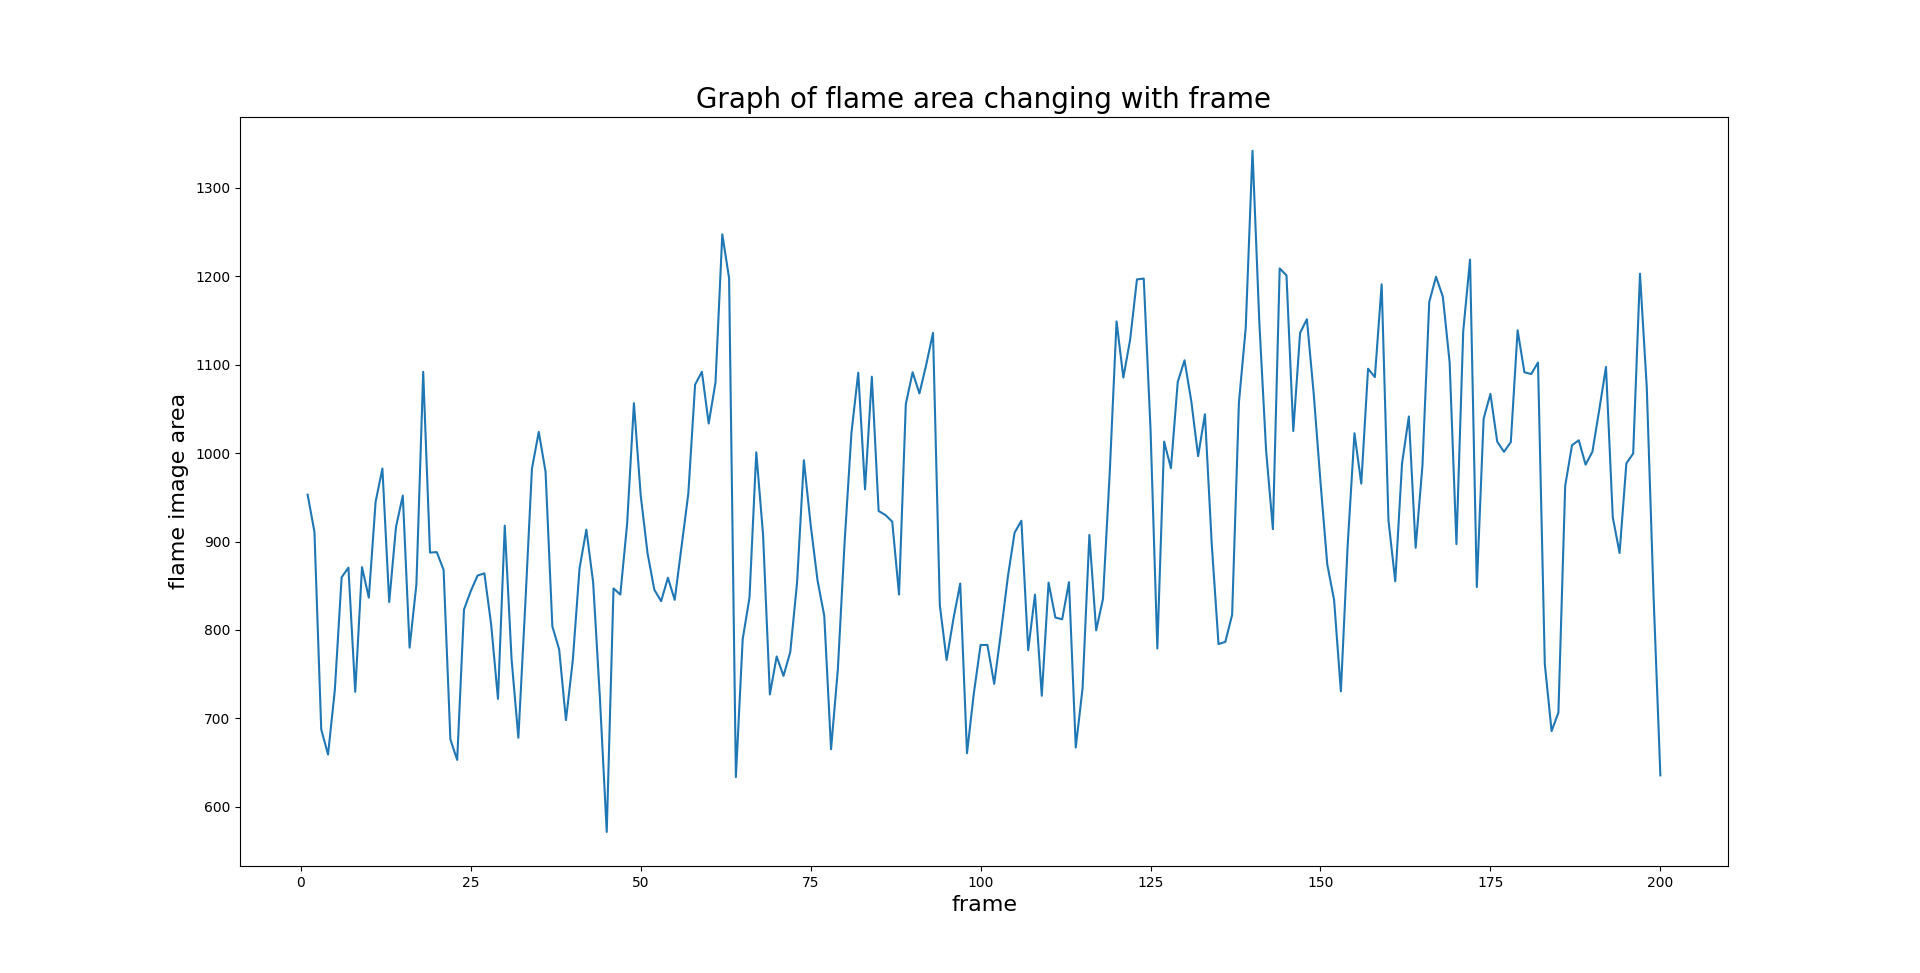
\includegraphics[width=\textwidth]{figures/extract_flicker_01.png}
      \caption{傅里叶变换前}
      \label{8}
    \end{figure}
    
    \begin{figure}[ht]
        \centering
        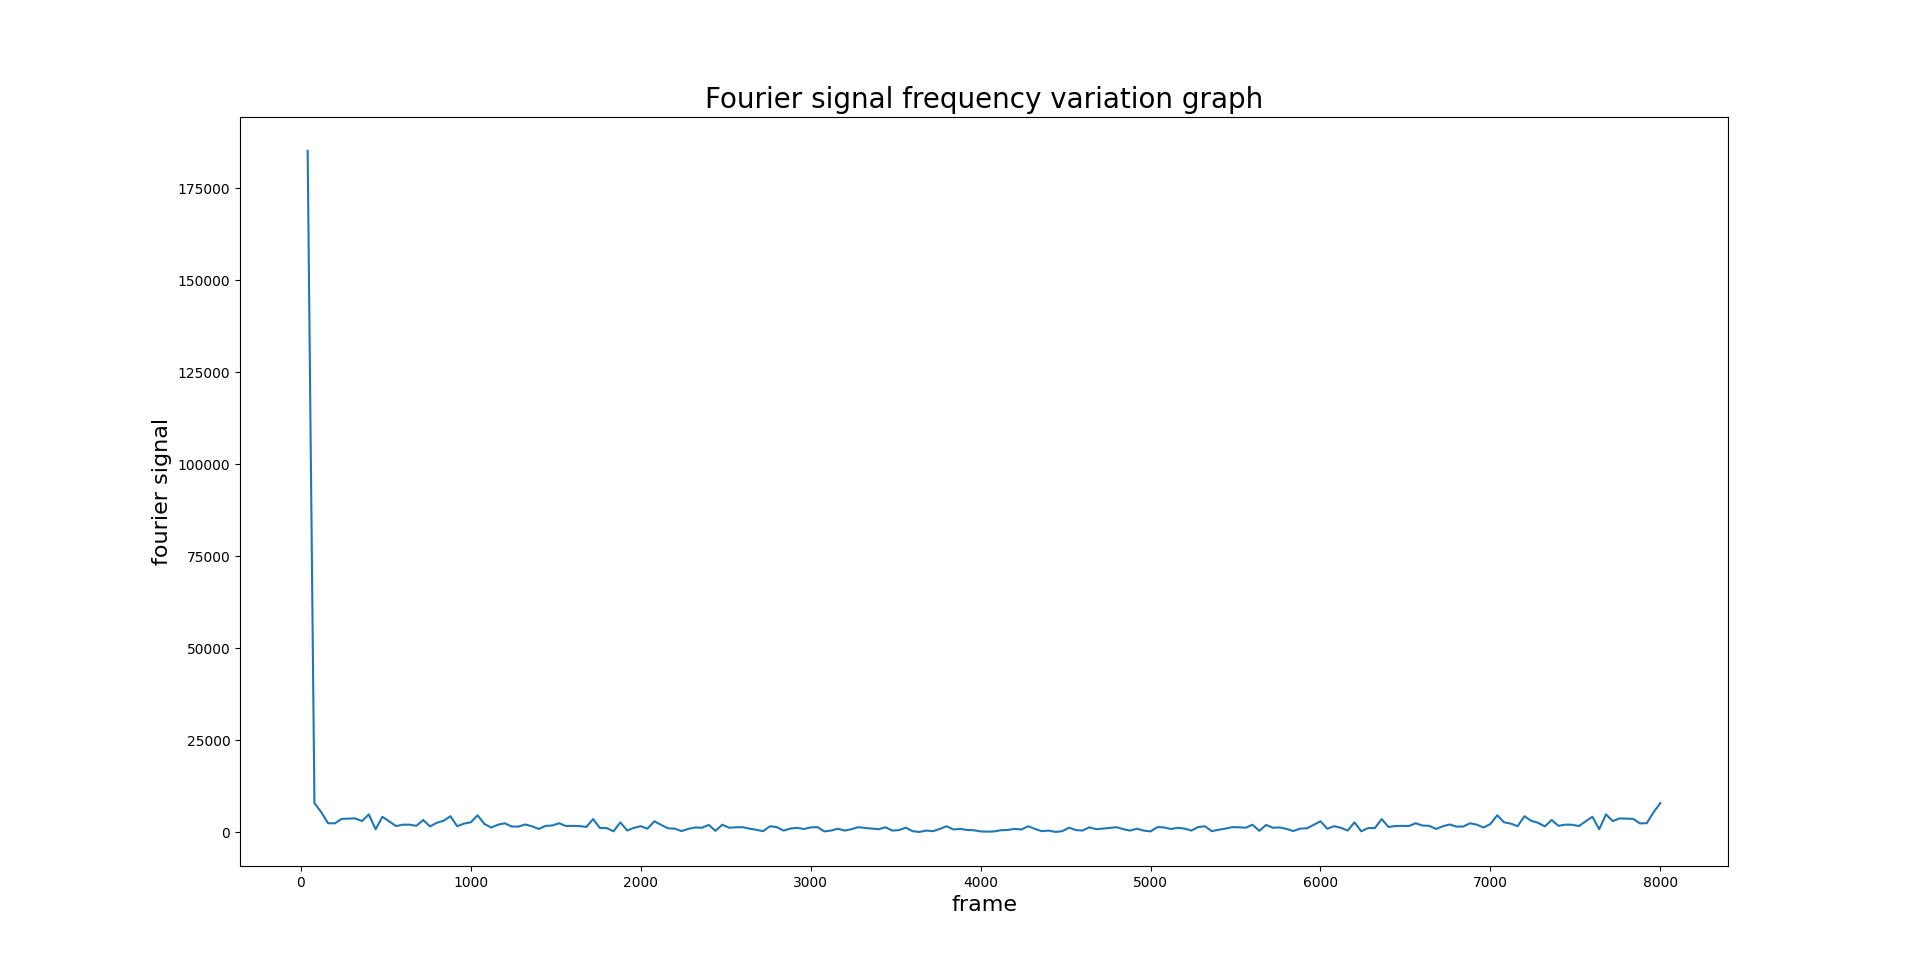
\includegraphics[width=\textwidth]{figures/extract_flicker_02.png}
        \caption{傅里叶变换后}
        \label{9}
    \end{figure}
    

依据展示可以看到,与目前研究现状吻合,变换前后都是震荡非线性的信号,肉眼难以捕捉到相关的信息,暂时不考虑使用。

\subsubsection{火焰形心变化}
火焰的形心变化是指火焰在燃烧过程中形心坐标位置的变化。形心是指火焰区域的质心或重心,对于图像来讲,就是火焰区域所有像素的中心。
一般来讲,燃烧的前期火焰会发生相对比较大的移动,中后期会趋于平稳,根据火焰的这一特性,我们可以通过对图像形心移动的相关的分析,
来排除相关的移动物体干扰源,从而防止对车辆,移动光源等的误报,这是火焰识别算法中一项重要的排除干扰参数指标。

这里我们可以对每个事件帧的图象像素中心进行统计,展示如\ref{10},\ref{11}(前5s)。
\begin{figure}[ht]
    \centering
    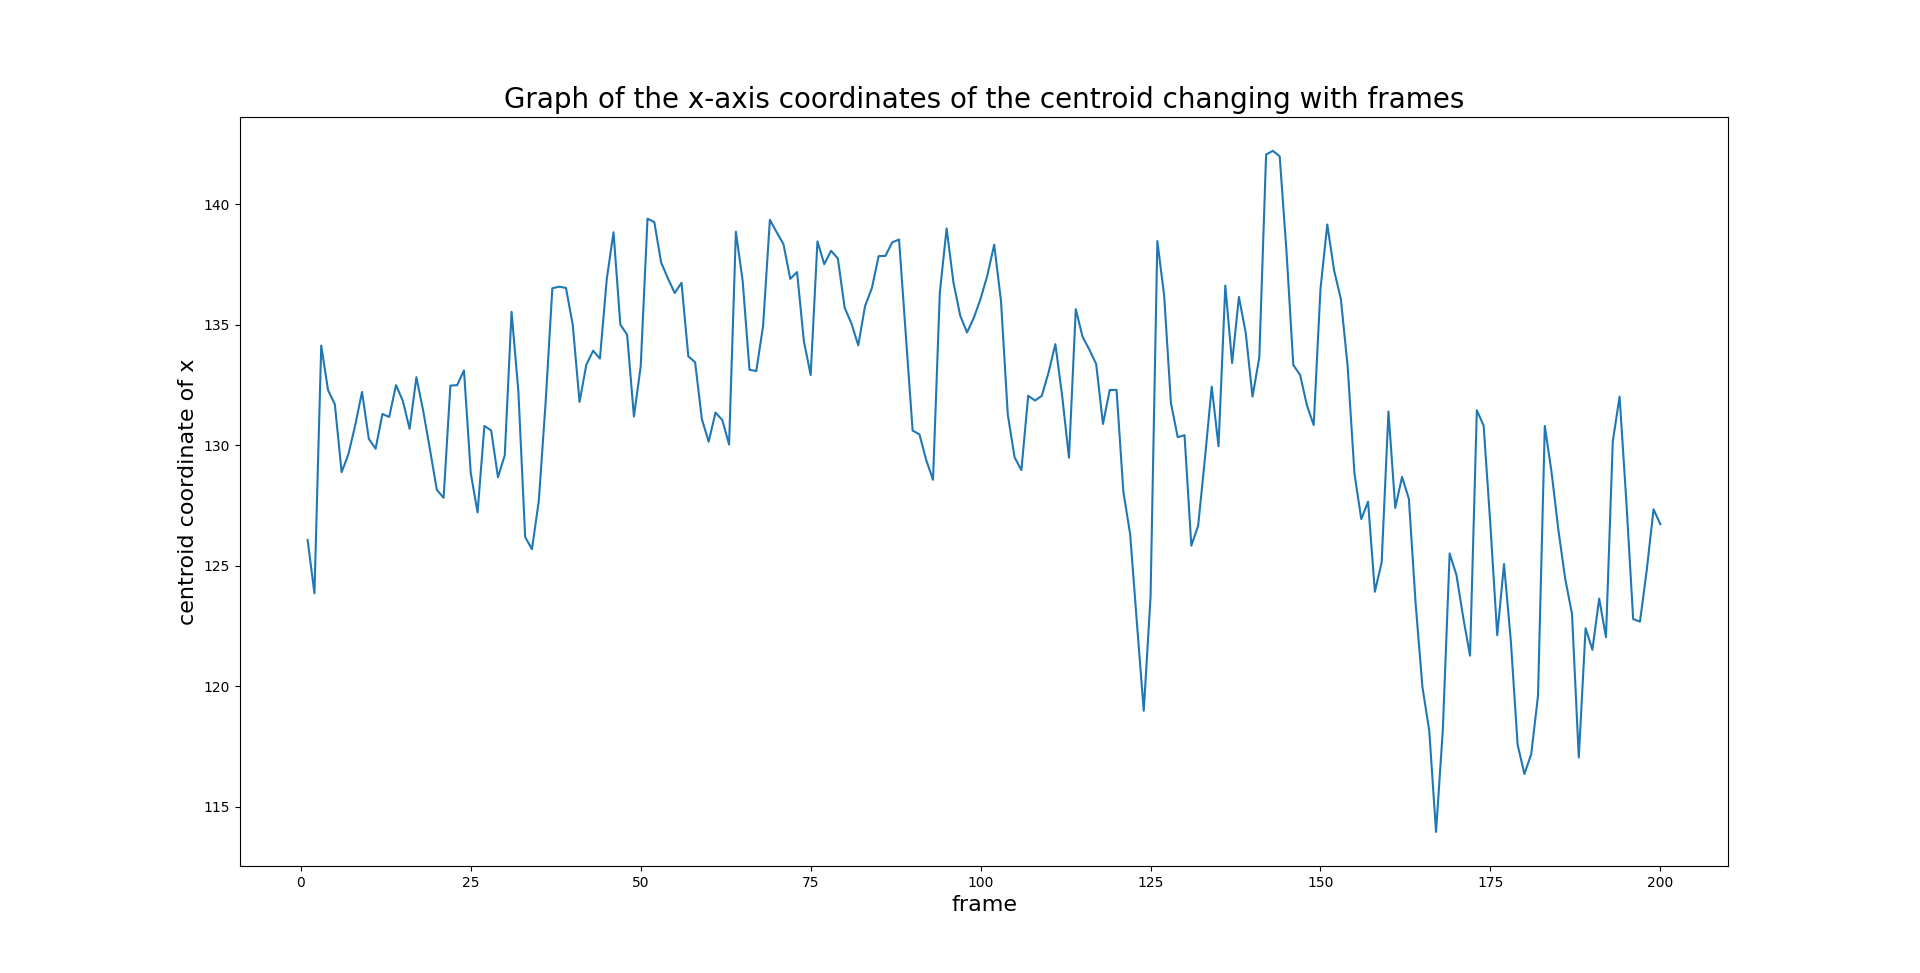
\includegraphics[width=\textwidth]{figures/extract_centroid_x.png}
    \caption{X轴方向(水平)}
    \label{10}
    \end{figure}

\begin{figure}[ht]
    \centering
    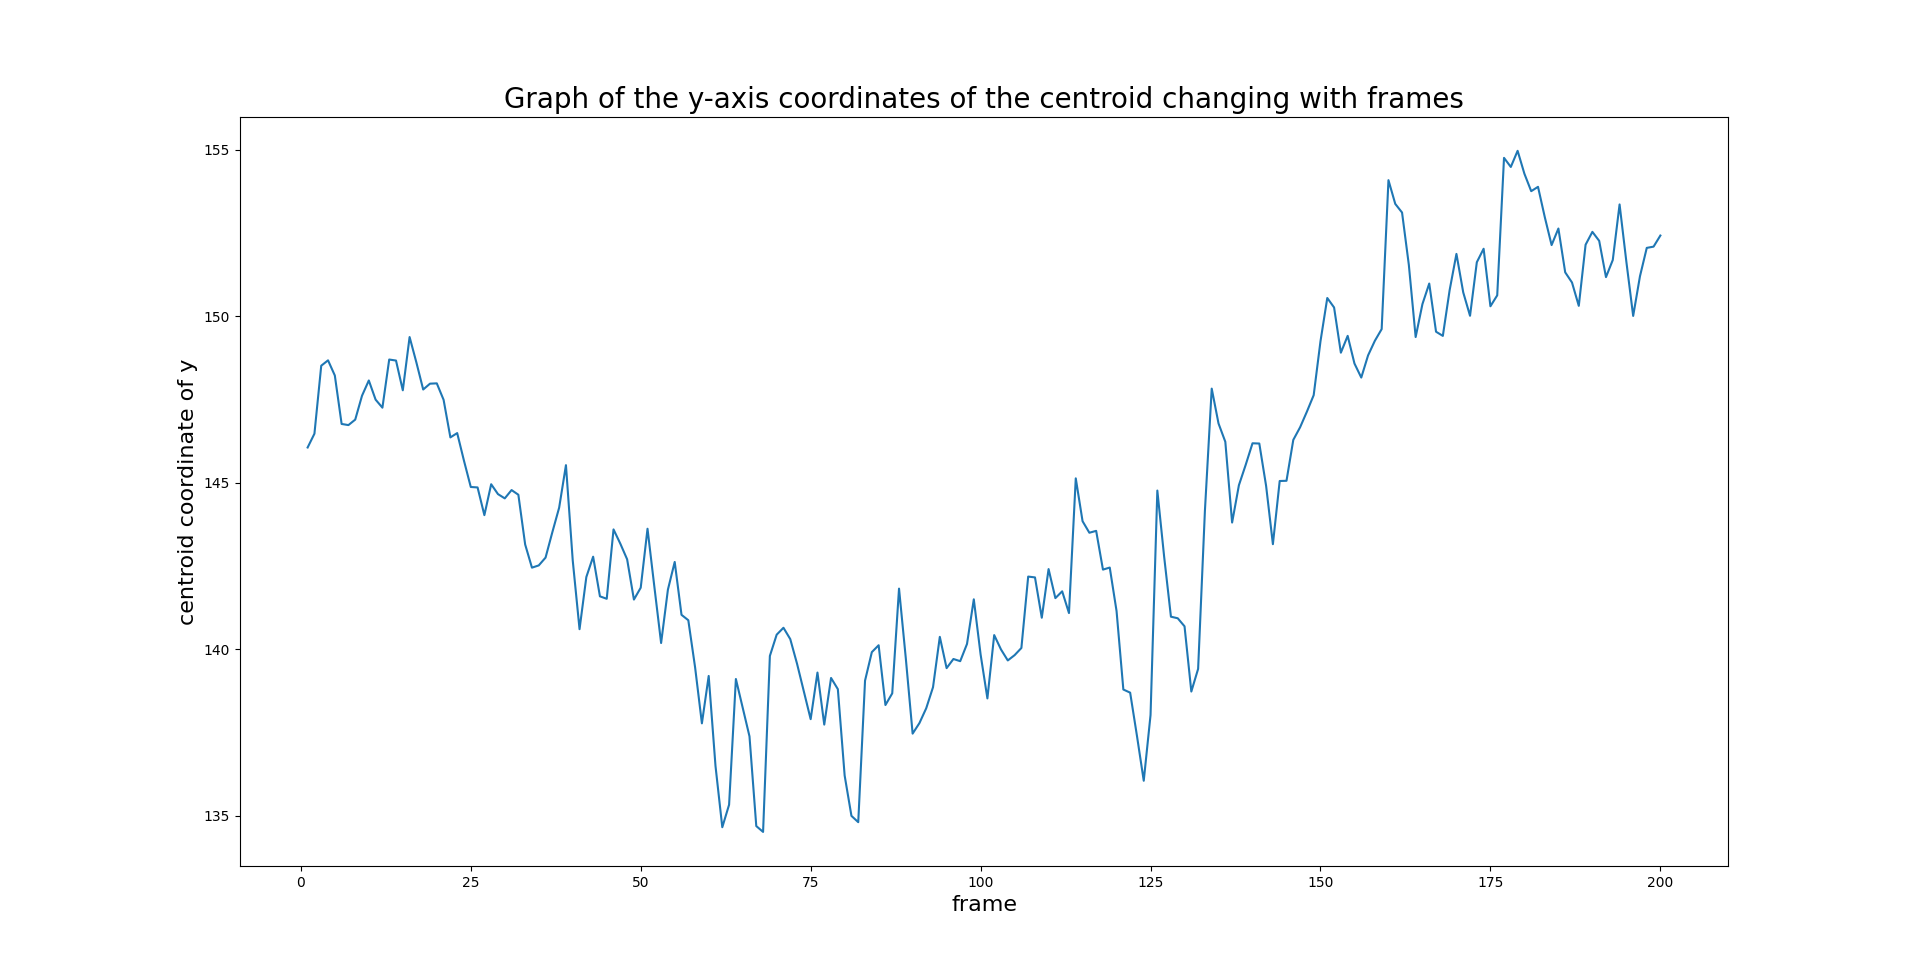
\includegraphics[width=\textwidth]{figures/extract_centroid_y.png}
    \caption{Y轴方向(垂直)}
    \label{11}
\end{figure}

形心坐标的波动情况与实验环境的联系较为紧密,例如当天的风向会影响x方向上的波动,材料的形状结构会影响y方向上的波动,
但是对于同一地点相同实验条件下的火焰来讲,其相对变化基本上遵循火焰特性。

\subsubsection{火焰面积生长系数}
火焰面积生长系数是指火焰在燃烧过程中火焰表面积随时间增长的比率。它是描述火焰在燃烧过程中扩展速度的一个重要参数,火焰面积生长系数可以用以下公式表示:
\begin{equation} 
    growth=\frac{dA}{Adt}
\end{equation}

其中,$\frac{dA}{dt}$是单位时间间隔内火焰面积变化量,A是当前面积。

对于我们的事件帧来说,固定每搁33ms进行取样,我们可以通过对比相邻两幅图像的面积,并计算前N幅图像面积的均值,即可获得火焰面积相对连续增长的特征,公式如下:
\begin{equation} 
    growth=N\frac{S_{i+1}-S_i}{\sum_{i=0}^{N}S_i}
\end{equation}

火焰面积生长系数反映了火焰燃烧过程中火焰表面积的增长速度,与火焰的燃烧速率密切相关,随着火灾的发展,燃烧速率增加时,火焰表面积增长的速度也会增加,火焰面积生长系数也会呈现增大的趋势,而火灾发展到中后期,其也会变的相对稳定
这里我们可以对事件帧的生长系数进行统计,效果展示如\ref{12},\ref{13}。
\begin{figure}[ht]
    \centering
    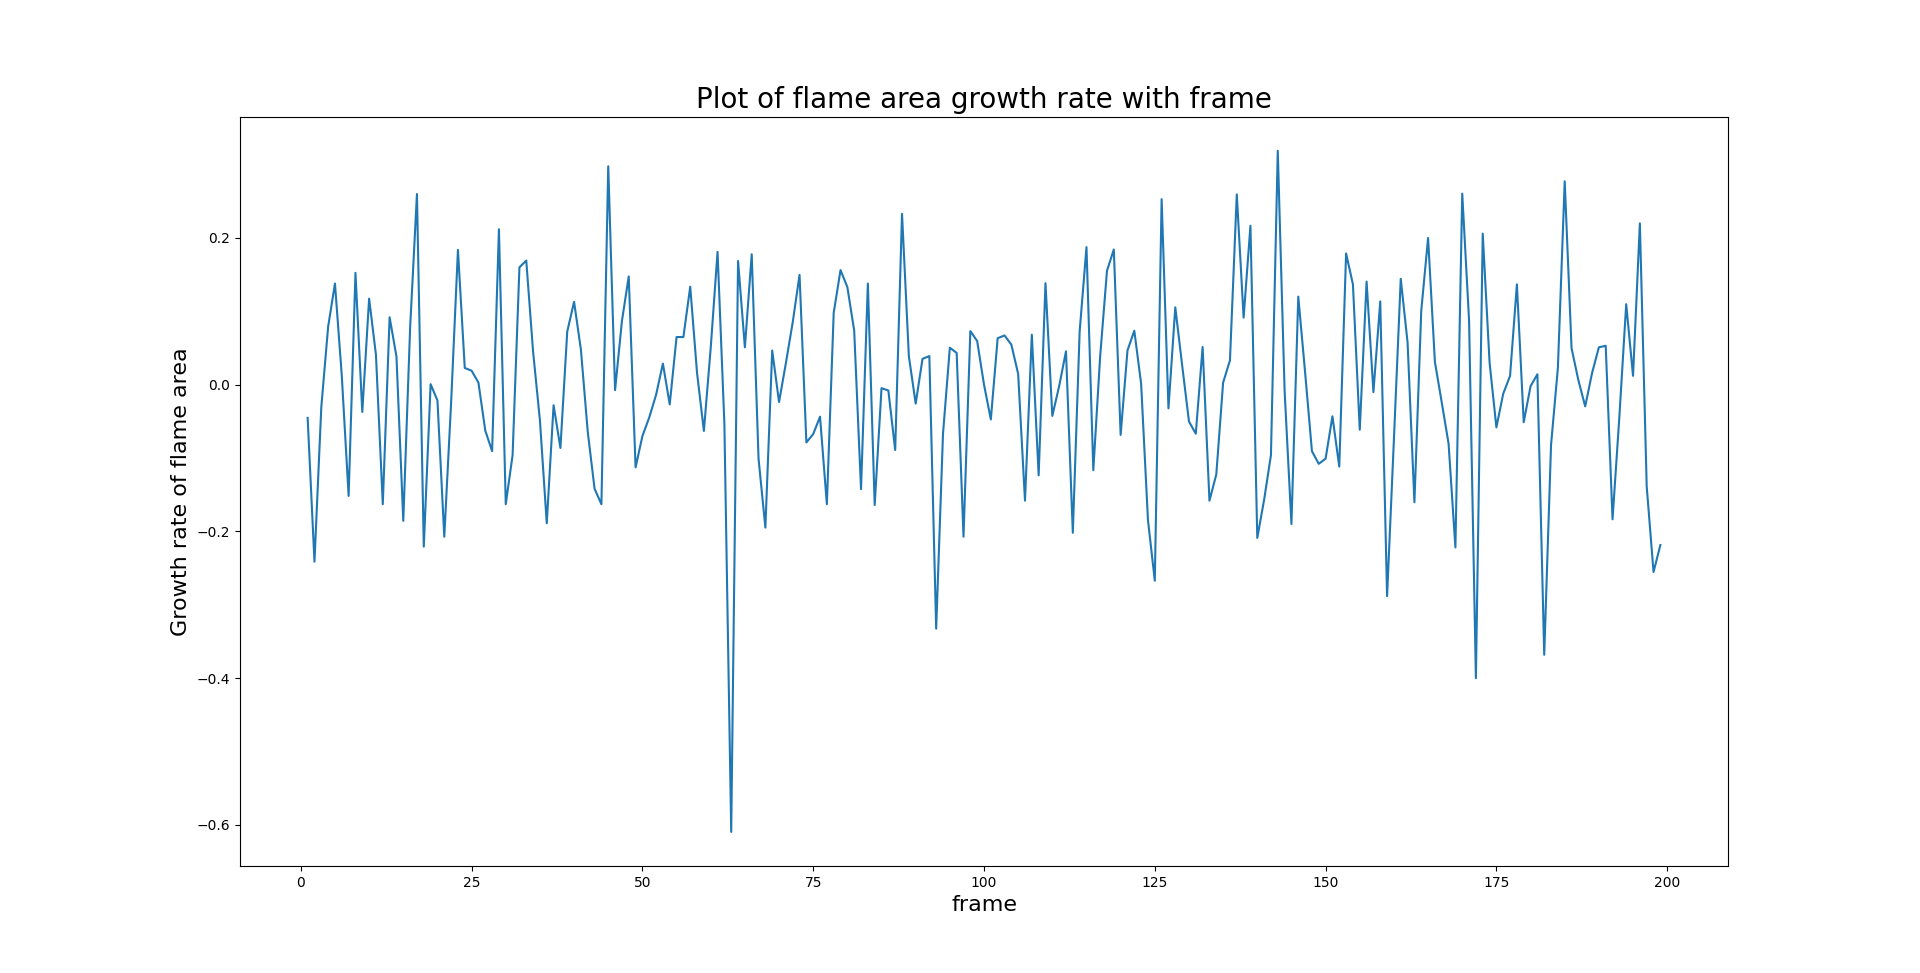
\includegraphics[width=\textwidth]{figures/extract_area_01.png}
    \caption{0-5s面积生长系数变化}
    \label{12}
\end{figure}

\begin{figure}[ht]
        \centering
        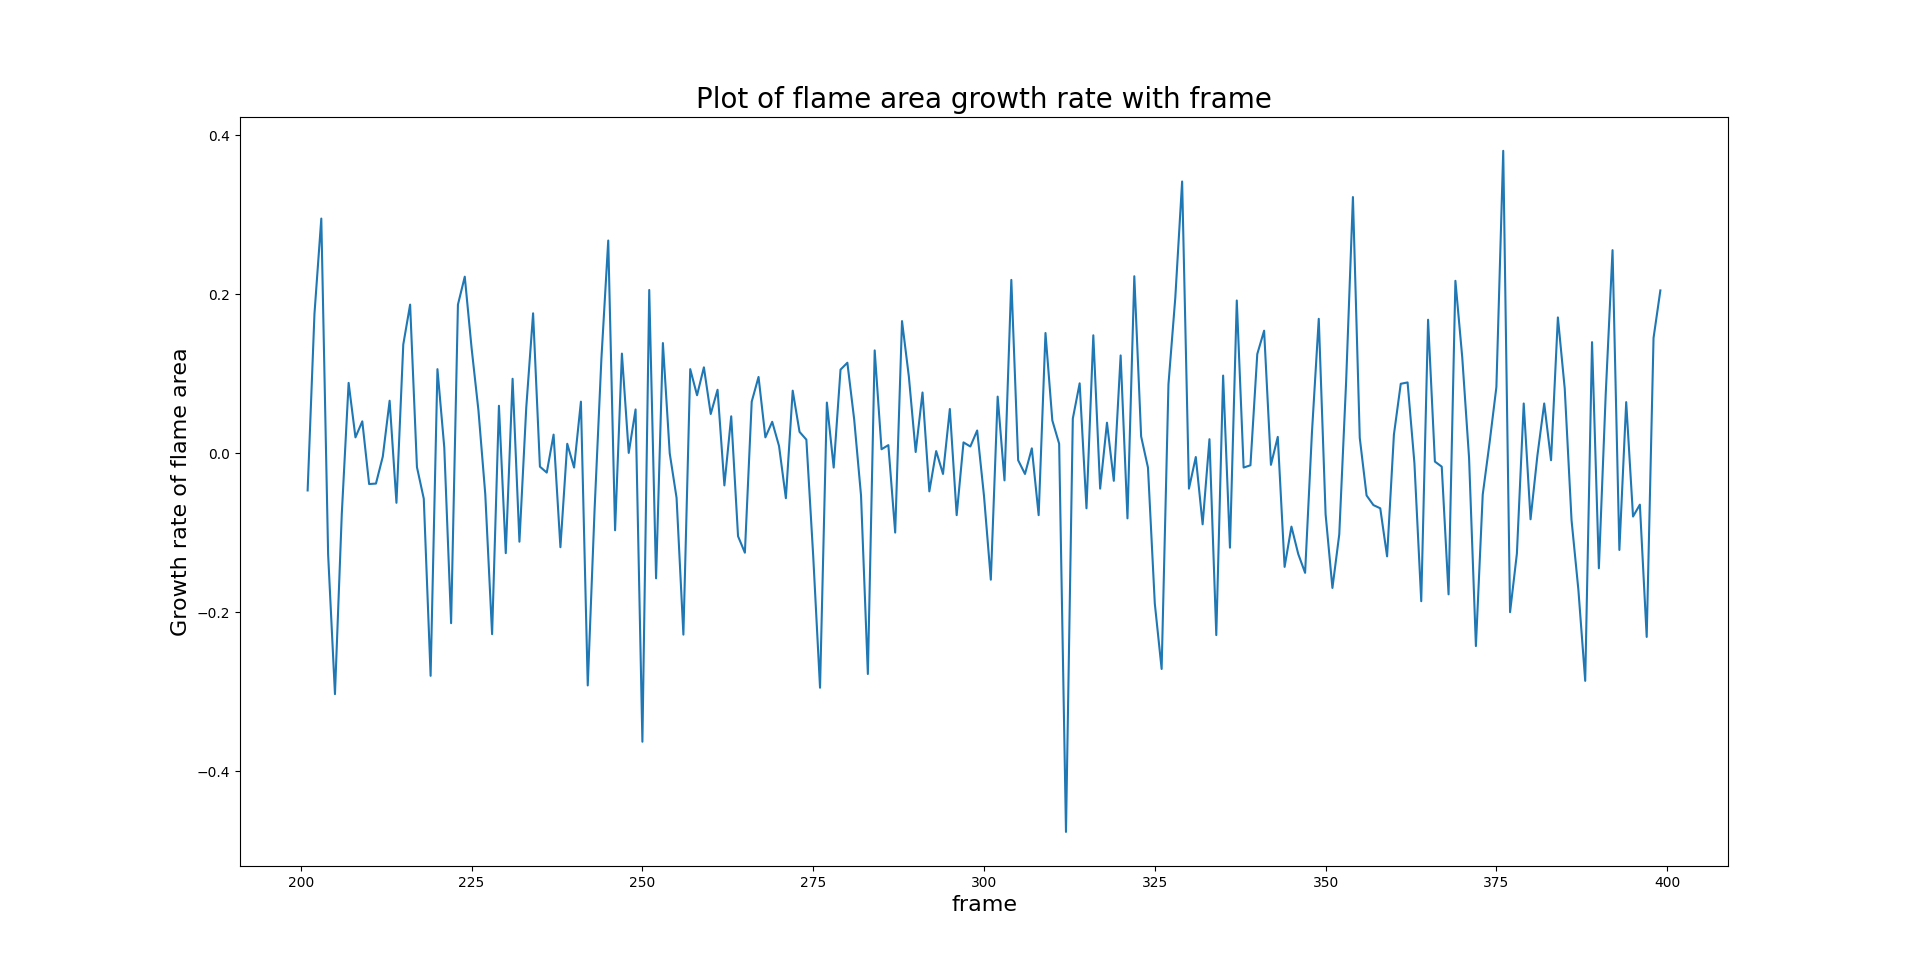
\includegraphics[width=\textwidth]{figures/extract_area_02.png}
        \caption{5-10s面积生长系数变化}
        \label{13}
\end{figure}

\section{本章小结}
本章我们主要介绍了本次工作中使用事件相机对火焰图像中所呈现出的动态与静态特征进行提取的过程,这些特征是用于区分火焰图象与其他常见干扰源图象的
主要依据,如何根据实验与环境条件选择与使用最具区分性的特征维度也是极为重要的。我们根据事件相机的特点对传统的一些特征进行了重新定义或引入,同时
也进行了相关的分析,后面的章节,我们将在这些特征的基础上,采用机器学习的思路,利用支持向量机尝试对火焰与非火焰进行初步区分,建立火焰检测算法模型与高维二分类空间,同时也会进行精确度评估与视觉效果比较。